% -----------------------------------------------------------------------
% --- DOCUMENT ---
% -----------------------------------------------------------------------

\documentclass[11pt, a4paper, french]{article}



% -----------------------------------------------------------------------
% --- PACKAGE ---
% -----------------------------------------------------------------------
\usepackage[french]{babel}

% Font
\usepackage[utf8]{inputenc}
\usepackage[T1]{fontenc}

% Marge du document
\usepackage[top=2cm, bottom=2cm, left=2cm, right=2cm]{geometry}

% Gérer les positionnement d'images
\usepackage{float}

% Import de fichier externe
\usepackage{graphicx}

% Mise en forme des URL
\usepackage{url}

% Informations sur un document compilé en PDF et les liens externes / internes
\usepackage{hyperref}

% Mise en page des tableaux
\usepackage{array}
\usepackage{tabularx}

% Espacement entre les lignes
\usepackage{setspace}

% Modifier la mise en page de l'abstract
\usepackage{abstract}

%pour utiliser \floatbarrier
%\usepackage{placeins}
%\usepackage{floatrow}



% -----------------------------------------------------------------------
% --- INFORMATION ET REGLES ---
% -----------------------------------------------------------------------

% Information sur le document
\hypersetup{							
    pdfauthor = {
        Edward Ransome, 
        Guillaume Milani, 
        Mathieu Monteverde, 
        Michael Spierer,
        Sathiya Kirushnapillai},                    % Auteurs
    pdftitle = {GEMMS - Edtieur d'image},           % Titre du document
    pdfsubject = {Mémoire de Projet},               % Sujet
    pdfkeywords = {Tag1, Tag2, Tag3, ...},          % Mots-clefs
    pdfstartview={FitH}}                            % ajuste la page à la largueur de l'écran
%pdfcreator = {MikTeX},                             % Logiciel qui a crée le document
%pdfproducer = {}}                                  % Société avec produit le logiciel



% -----------------------------------------------------------------------
% --- DEBUT DU DOCUMENT ---
% -----------------------------------------------------------------------
\begin{document}
    
\selectlanguage{french} 

% Espacement entre les lignes
\newcommand{\HRule}{\rule{\linewidth}{0.5mm}}

% Page de garde
\begin{titlepage}
    \begin{center}
        % Upper part of the page. The '~' is needed because only works if a paragraph has started.
        % \includegraphics[width=0.35\textwidth]{./logo}~\\[1cm]
        
        \textsc{\LARGE Haute Ecole d'Ingénierie et de Gestion du Canton de Vaud (HEIG-VD)}\\[1.5cm]
        
        \textsc{\Large }\\[0.5cm]
        
        % Title
        \HRule \\[0.4cm]
        
        {\huge \bfseries Projet de semestre (PRO)\\
            Editeur d'image GEMMS \\[0.4cm] }
        
        \HRule \\[1.5cm]
        
        % Author and supervisor
        \begin{minipage}{0.4\textwidth}
            \begin{flushleft} \large
                \emph{Auteur:}\\
                Edward \textsc{Ransome}\\
                Guillaume \textsc{Milani}\\
                Mathieu \textsc{Monteverde}\\
                Michael \textsc{Spierer}\\
                Sathiya \textsc{Kirushnapillai}
            \end{flushleft}
        \end{minipage}
        \begin{minipage}{0.4\textwidth}
            \begin{flushright} \large
                \emph{Client:} \\
                René \textsc{Rentsch}\\
                \emph{Référent:} \\
                René \textsc{Rentsch}\\
            \end{flushright}
        \end{minipage}
        
        \vfill
        
        % Bottom of the page
        {\large \today}
        
    \end{center}
\end{titlepage}


\newpage
~

\thispagestyle{empty}
\newpage

% \input{./abstract.tex}

\tableofcontents
\thispagestyle{empty}
\setcounter{page}{0}
%ne pas numéroter le sommaire

\newpage

%espacement entre les lignes d'un tableau
\renewcommand{\arraystretch}{1.5}
\setlength{\parskip}{1em}
\setlength{\parindent}{0pt}.

%====================== INCLUSION DES PARTIES ======================

~
\thispagestyle{empty}
%recommencer la numérotation des pages à "1"
\setcounter{page}{0}
\newpage

\section{Introduction}
GEMMS est un éditeur d'images réalisé en Java en se basant sur les fonctionnalités graphiques de JavaFX 8. Il a été réalisé dans le cadre de la branche PRO (Projet de semestre) de la deuxième année d'informatique logicielle de la Haute-École d'Ingénierie et Gestion du canton de Vaud (HEIG-VD). 
Le programme a été élaboré sur une durée de 14 semaines aboutissant le 31 Mai 2017.

\section{Objectif}
L'application GEMMS a été conçue pour éditer des images de manière rapide, simple et intuitive. Le programme ne nécessite pas d'apprentissage particulier, comme certains programmes plus lourds comme Adobe Photoshop ou encore GIMP.

L'interface est propre, avec des icônes représentant les différents outils et actions possibles dans le programme en essayant de minimiser les menus déroulants surchargés. Des infobulles donnent une description concise de chaque outil lorsqu'on passe la souris dessus.

Bien que plus simple que les applications lourdes mentionnées ci-dessus, un concept très important dans l'édition d'image, les calques, est conservé. Certains éditeurs très basiques comme Paint sous Windows ne fournissent pas cette fonctionnalité. Les calques permettent de superposer des images, du texte, ou des canevas et de les déplacer, modifier ou effacer indépendamment les uns des autres. Lors de l'exportation du projet vers un format image, les calques sont aplatis et l'image est exportée en perdant ces informations.

Un projet GEMMS ne peut cependant pas uniquement être exporté en tant qu'image, mais sauvegardée dans un fichier de projet \og.gemms \fg{}. Ce type de fichier peut être ouvert par l'application pour restaurer tout le projet en cours, recréant chaque calque ainsi que les transformations effectuées dessus.

\section{Conception \& Architecture}
\subsection{Technologies utilisées}
\subsubsection{Java 8}
Parmi les deux langages de haut niveau proposés pour l'élaboration de ce projet (Java ou C++), nous avons choisi Java pour sa portabilité, sa sécurité et ses performances. De plus, la dernière version de Java propose la librairie graphique JavaFX qui correspond en tout point à notre projet. Enfin, notre équipe est également plus habile à programmer à l'aide du langage Java.

\subsubsection{JavaFX 8}
JavaFX, successeur de Swing, est la librairie de création d'interface graphiques officielle de Java. La version 8, utilisée pour ce projet, ajoute de nouvelles fonctionnalités et est la plus récente version utilisable avec Scene Builder.

\begin{figure}[h]
    \caption{Architecture de JavaFX}
    \centering
    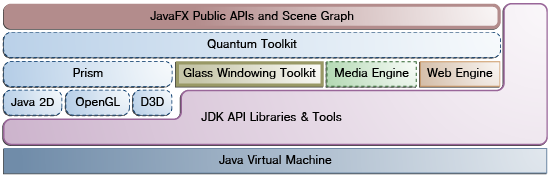
\includegraphics[width=\textwidth]{arch_javafx.png}
    \label{fig:arch_javafx}
\end{figure}

Comme vous pouvez le voir sur la figure \ref{fig:arch_javafx}, BLA BLA BLA A COMPLETER, A PARLER DE CSS ETC


\subsubsection{Scene Builder 8.3.0}
Scene Builder de Gluon permet de manipuler des objets JavaFX graphiquement et exporter ceux-ci dans un fichier .fxml interprétable par la librairie graphique. L'interface de base à été conçue lors de l'élaboration du cahier des charges pour présenter un exemple de l'interface de l'application finale. Plusieurs mock-ups ont été présentés et c'est sur ceux-cis que nous nous sommes basés pour construire, grâce à Scene Builder, une base d'interface sur la laquelle nous avons rajouté des composants et fonctionnalités tout au long de l'élaboration de l'application. La flexibilité de JavaFX permet d'ajouter des éléments via un fichier externe fxml mais aussi directement dans le code, ce que nous avons aussi utilisé.

\subsubsection{Maven}
Pour la compilation du projet et l'importation aisée de celui-ci dans un nouvel environnement de travail, nous avons utilisé l'outil Maven de Apache.
TODO TODO TODO TODO TODO COMPLETER

\subsubsection{Git}
Git est un logiciel de gestion de version utilisé pour permettre de stocker tous les fichiers du projet ainsi que toutes les modifications leur ayant été apportés depuis leur création. Pour chaque nouvelle fonctionnalité, nous avons procédé par la création d'une branche à partir de la branche principale (une version fonctionnelle du programme, contenant les fonctionnalités implémentées et testées). Ces nouvelles branches permettent de développer les fonctionnalités du programme indépendamment et de les ajouter à la branche principale une fois inspectées et testées par plusieurs membres de l'équipe.

\subsubsection{GitHub}
Github est un service web permettant de parcourir visuellement l'historique Git ainsi que de fournir des outils de gestion de Git. Notamment, pour chaque fonctionnalité ou chaque bug découvert, une "issue" (un problème) peut être ouverte et assignée à un ou plusieurs membres de l'équipe. Dès la fin de l'élaboration du planning de notre projet, des issues ont été assignées à chaque développeur. Celles-ci ont permis de mieux se fier au planning et toujours avoir en vue ce qu'il restait à implémenter.

\subsection{Comparaison de l'interface finale avec notre mock-up}
Le mock-up de l'interface à été conçu au début du projet en prenant compte de toutes les fonctionnalités que le programme devait fournir. Voici une comparaison de celui-ci avec l'interface finale.

\begin{figure}[H]
	\caption{Mock-up de l'interface}
	\centering
	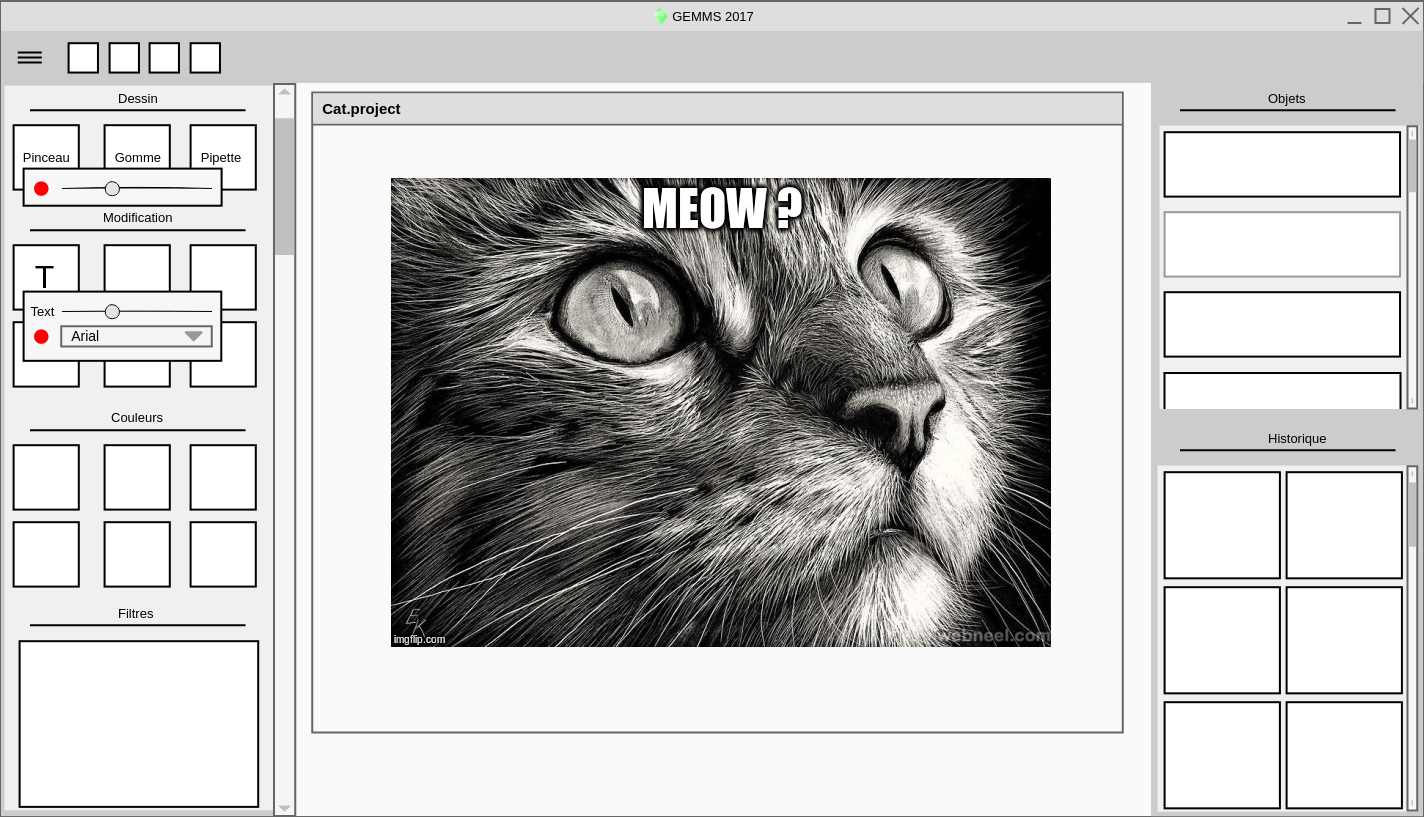
\includegraphics[scale=0.35]{Cat_MOCKUP.png}
	\label{fig:cat_mockup}
\end{figure}

\begin{figure}[H]
	\caption{Interface finale du programme}
	\centering
	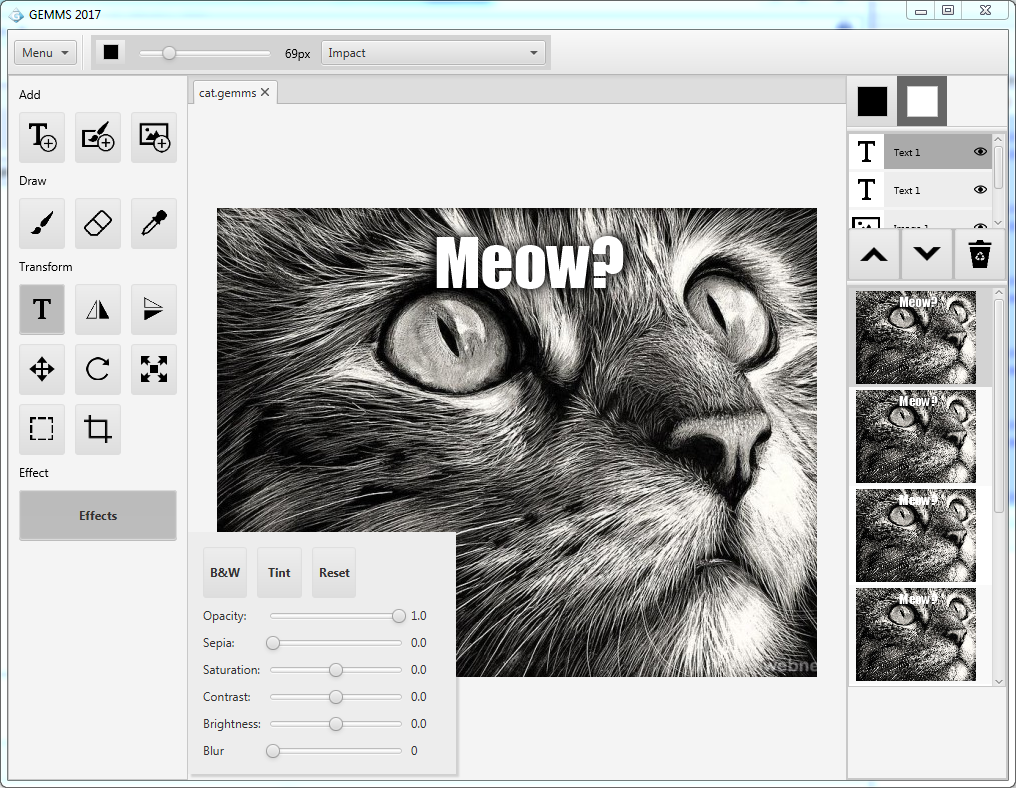
\includegraphics[scale=0.6]{Cat_GEMMS.PNG}
	\label{fig:cat_gemms}
\end{figure}

Comme le montrent les figures \ref{fig:cat_mockup} et \ref{fig:cat_gemms}, l'interface conçue lors de l'élaboration du cahier des charges à été repris presque entièrement pour notre programme. Les différences majeurs sont les paramétrages des outils, qui ont lieux en haut de l'interface à coté du menu déroulant, ainsi que les filtres \& effets, qui ont lieux dans une fenêtre qui peut être ouverte ou fermée à souhait pour rendre l'interface moins chargée. 
%
% \input{./besoins.tex}
%
% \input{./autre_partie.tex}
%
% \input{./resultats.tex}
%
% \input{./bilan.tex}
%
% \input{./annexes.tex}

\newpage

%récupérer les citation avec "/footnotemark"
\nocite{*}

%choix du style de la biblio
\bibliographystyle{plain}
%inclusion de la biblio
\bibliography{bibliographie.bib}
%voir wiki pour plus d'information sur la syntaxe des entrées d'une bibliographie

\end{document}
